\documentclass[a4paper]{article}
\usepackage{tabularx}
\usepackage{geometry}
\geometry{
  a4paper,
  total={170mm,257mm},
  left=17mm,
  top=20mm,
   }

\usepackage{polski}
\usepackage[utf8]{inputenc}
\usepackage{url}
\usepackage{graphicx}
\usepackage[font=small,labelfont=bf]{caption}
\usepackage{wrapfig}

\setlength{\parskip}{0pt}
\setlength{\parindent}{0pt}

\title{\emph{Calineczka\\ \small last update 2022.03.21 \normalsize}}
\date{}

\begin{document}

\maketitle

\section*{Info}

\emph{Calineczka} -- Ścisław Dercz (born Michał Jędrzej Stańczyk, 1984 in Gdańsk, Poland).
Exploring boundary cases of music with analog synthesizers since 2014.
%From 2002 to 2007 known as \emph{Aleph}.
Runs a cassette label \emph{important drone records}.


\vspace{4mm}
%\url{https://soundcloud.com/drcz}\\
\url{http://drcz.github.io/calineczka.html}\\
\url{https://www.discogs.com/artist/5994202-Calineczka}\\
\url{http://importantdronerecords.bandcamp.com}\\

\vspace{7mm}

\section*{Projects and collaborations}

\begin{wrapfigure}[8]{r}{0.26\textwidth}
  \vspace{-5mm}
  \centering
  \includegraphics[width=0.26\textwidth]{w-sfini-conditions.jpg}
  %\includegraphics[width=\linewidth]{w-sfini-conditions.jpg}
  %\vspace{-15mm}
\end{wrapfigure}

From 2002 to 2007 active as \emph{Aleph}, a drone/noise act. Often playing in collaboration with \emph{Artur ARh+ Kwiatkowski} (\emph{Pure}, currently \emph{Akton} and a half of \emph{DREN}) and \emph{Non-Iron Group} (\emph{Robert Sochacki}, \emph{Zambari}, \emph{Anna Patrini}, \emph{Arszyn} \emph{et al.}).
Did a ``correspondence'' album with German \emph{Eternal Ice}.
%Positively reviewed and played by a few underground radio podcasts.

\vspace{4mm}

From 2004 to 2005 member of garage dark ambient band \emph{Muezinn} with \emph{Grzegorz Kwiatkowski} (currently \emph{Trupa Trupa}).
In 2005 member of a short-lived cutup/collage guerrilla \emph{Szrómberrypłot} with \emph{Jakub Bilski} tossing recycled cassettes to random mailboxes and public toilets.

\vspace{7mm}

\begin{wrapfigure}[5]{l}{0.26\textwidth}
  \vspace{-5mm}
  \centering
  \includegraphics[width=0.26\textwidth]{bzss-paracetamol.jpg}
  %\vspace{-15mm}
\end{wrapfigure}

\vspace{4mm}

From 2006 to 2007 member of d'n'b cabaret \emph{Boa Zeria Sound System / BZSS} with \emph{Rafał ``Siebenlustigetomaten'' Zaremba} (weird performances and short films\footnote{Some stranger saved a copy of one: \url{https://www.youtube.com/watch?v=RpXXtEzkD2w}}).

\vspace{4mm}
Since 2010 member of dada-drone duo \emph{Bracia Feccaliano} with \emph{Marek P.} (over a dozen lengthy compositions on classified recycled cassettes).

\vspace{13mm}

\begin{wrapfigure}[4]{r}{0.26\textwidth}
  \vspace{-5mm}
  \centering
  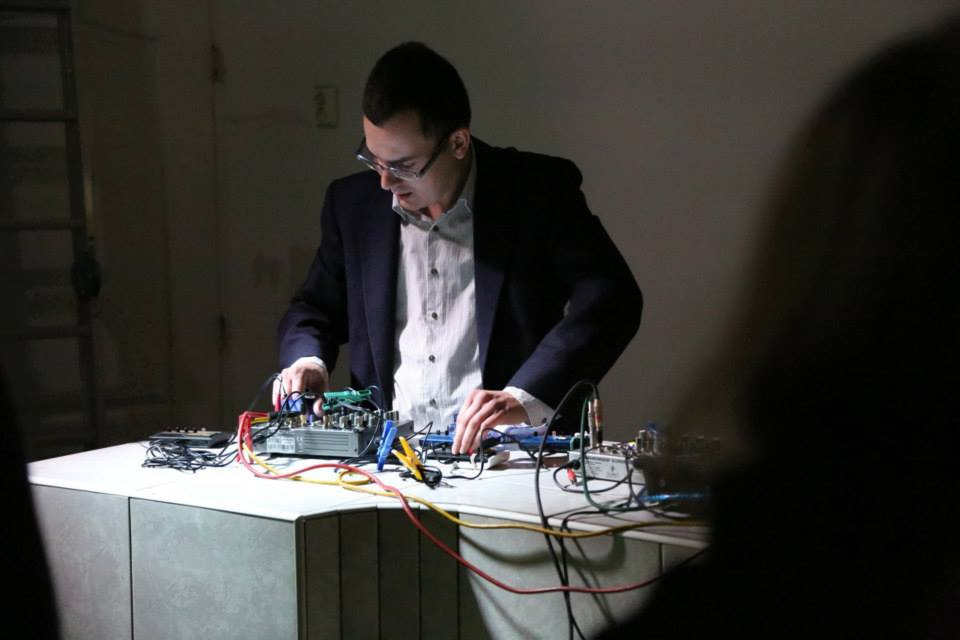
\includegraphics[width=0.26\textwidth]{calineczka-street.jpg}
\end{wrapfigure}

Late 2013 started explorations of boundary cases of composition using analog synthesizers, in 2014 taking the name \emph{Calineczka} (Polish for ``Thumbelina'').

\vspace{4mm}
On September 2017 on a tour\footnote{\url{https://soundcloud.com/drcz/sets/four-and-a-half-rds4s-one-rds3-and-one-rds6}} with \emph{Dawid ``Purgist'' Kowalski} performed also as a duo \emph{Psychotronika} (drone/experimental).
%In parallel to the tour played his almost 5h long live composition ``RDS-6''\footnote{\url{https://soundcloud.com/drcz/20170824-rds-6-kolonia-artystow-gdansk}}.

\vspace{4mm}
On December 21 2018 started \emph{important drone records}.

\vspace{4mm}
On April 2019 joined \emph{Libet}.


\newpage

\section*{Performances\footnote{\emph{N.b.} all venues located in Poland unless stated otherwise.}}

\vspace{4mm}
\textbf{as Calineczka:}

\vspace{2mm}

\begin{tabularx}{\textwidth}{r l}
\hline
2020-02-02 & ``RDS-4'' (Soundscapism vol.30) $@$ The Banshee Labyrinth, Edinburgh, UK \\
\hline
2020-02-01 & ``RDS-4'' (Liminal Haze/Calineczka tour) $@$ The Soundroom, Gateshead, UK \\
\hline
2020-01-31 & ``RDS-5'' (Liminal Haze/Calineczka tour) $@$ AME's Dai Hall, Huddersfield, UK \\
\hline
2020-01-30 & ``RDS-4'' (Liminal Haze/Calineczka tour) $@$ Fuel Cafe Bar, Mancherster, UK \\
\hline
2019-10-02 & ``RDS-5'' (Modelbau/Calineczka) $@$ Albert van Abbehuis, Eindhoven, NL \\
\hline
2019-09-29 & ``RDS-5'' (Soundscapism vol.28) $@$ The Banshee Labyrinth, Edinburgh, UK \\
\hline
2019-02-15 & ``RDS-9'' (Ruisburo) $@$ de Ruimte, Amsterdam, NL \\
\hline
2019-01-26 & ``RDS-9'' (Drone, Noise, No Ambient) $@$ Kolonia Artystów, Gdańsk \\
\hline
2019-01-25 & ``RDS-9'' (Noise 01.25) $@$ Przychodnia Skłot, Warszawa \\
\hline
2017-08-25 & ``Totskoye'' (Purgist/Calineczka/Psychotronika tour) $@$ Mózg, Bydgoszcz \\
\hline
2017-08-24 & ``RDS-4'' (Purgist/Calineczka/Psychotronika tour) $@$ Kolonia Artystów, Gdańsk \\
\hline
2017-08-24 & ``RDS-6'' (a 5h composition) $@$ Kolonia Artystów, Gdańsk \\
\hline
2017-08-23 & ``RDS-4'' (Purgist/Calineczka/Psychotronika tour) $@$ Kij, Łódź \\
\hline
2017-08-22 & ``RDS-4'' (Purgist/Calineczka/Psychotronika tour) $@$ Ch25, Warszawa \\
\hline
2017-08-21 & ``RDS-3'' (Purgist/Calineczka/Psychotronika tour) $@$ Wonle Tory TSA, Bytom \\
\hline
2017-08-19 & ``RDS-4'' (Purgist/Calineczka/Psychotronika tour) $@$ Teatr Cinema, Michałowice \\
\hline
2017-05-01 & ``RDS-2'' (international labour day) $@$ Kolonia Artystów, Gdańsk \\
\hline
2014-05-31 & ``RDS-1'' $@$ Streetwaves festival, Gdańsk \\
\end{tabularx}

\vspace{11mm}

\textbf{As Aleph/alef:}

\vspace{2mm}

\begin{tabularx}{\textwidth}{r l}
\hline
2007-10-05 & Non Iron Group (Robert Sochacki, Anna Patrini, Jerzy Mazzol, Arszyn, alef)\\
           & $@$ Non Iron Festival, klub Sfinks, Sopot\\
\hline
2007-03-09 & alef $@$ ``noizzy pigs'' festival, klub Pilon, Toruń\\
\hline
2006-03-25 & Aleph $@$ pgr\_art (Kolonia Artystów), Gdańsk\\
\hline
2005-12-06 & ``noise performance screaming'' (Patrini, Sochacki, Aleph) $@$ Stacja deLuxe, Gdańsk\\
\hline
2005-11-20 & neodadanoise (Sochacki, Patrini, Aleph) $@$ klub Mandarynka, Sopot\\
\hline
2005-10-29 & ``stany/conditions'' exhibition (Robert Sochacki, Aleph, Partini, Zambari) $@$ pracownia3, Warszawa\\
\hline
2005-10-28 & ``stany/conditions'' exhibition (Robert Sochacki, Aleph, Partini) $@$  pracownia3, Warszawa\\
\hline
2005-10-27 & ``stany/conditions'' exhibition (Robert Sochacki, Aleph) $@$ pracownia3, Warszawa\\
\hline
2005-10-15 & ``stany/conditions'' exhibition (Robert Sochacki, Aleph, Zambari) $@$  Teatr Znak, Gdańsk\\
\hline
2005-09-01 & ``stany/conditions'' exhibition (Robert Sochacki, Aleph) $@$ klub Sfinks, Sopot\\
\hline
2005-05-20 & Freistadtjugend (Aleph \& ARh+) $@$ pgr\_art (Kolonia Artystów),  Gdańsk\\
\hline
2005-04-02 & Freistadtjugend (Aleph \& ARh+) $@$ ``Rytualne oblicza kontrkultury'' festival, Dom Muz, Toruń\\
\hline
2005-02-19 & Freistadtjugend (Aleph \& ARh+) $@$ pgr\_art (Kolonia Artystów),  Gdańsk\\
\hline
2005-01-09 & the incredible h34Dsh0t b0yZ (Aleph vs ARh+) $@$ Klub Orbital, Gdańsk\\
\hline
2004-11-19 & Aleph \& ARh+ $@$ Wolna Pracownia pgr\_art (Kolonia Artystów), Gdańsk\\
\hline
2004-11-12 & Aleph $@$ ``tripolis 8'' festival, klub Sfinks, Sopot\\
\hline
2004-07-25 & Aleph $@$ ``day out of time'' festival, Smętowo Graniczne\\
\end{tabularx}

\vspace{11mm}

\textbf{As Boa Zeria Sound System:}

\vspace{2mm}

\begin{tabularx}{\textwidth}{r l}
\hline
2007-11-02 & \emph{``RORATY''} performance $@$ pgr\_art (Kolonia Artystów), Gdańsk\\
\hline
2007-04-28 & (support for Mikrowafle) $@$  pgr\_art (Kolonia Artystów), Gdańsk\\
\hline
2006-06-24 & BZSS $@$ ``elektrostrajk'' festival, pgr\_art (Kolonia Artystów), Gdańsk\\
\hline
2006-04-01 & \emph{``tańce i spiewi czyli audiowizualni szoł dla Ewi na dzień kobiet za talón''} performance,\\
           & $@$ pgr\_art (Kolonia Artystów), Gdańsk\\
\end{tabularx}


\newpage

\section*{Releases}

\textbf{As Calineczka:}

\vspace{2mm}

\begin{tabularx}{\textwidth}{l l l l l}
\hline
2022 & Untitled (track on comp. ,,Fermium'') & digital & 1834 & (ET-100)\\
\hline
2021 & Thank You For The Music & digital & 1834 & (ET-094)\\
     & (When The Music's Over) & & & \\
\hline
2020 & Subject With No Object & digital & Inner Space prod. & (IP-003) \\
\hline
2020 & kysztymska & microSD & Szara Reneta & (taśma dwudziesta\\
     &            &         &              & trzecia)\\
\hline
2020 & Audience & digital & 1834 & (ET-071)\\
\hline
2020 &  $\pi_1(S^1)$ (track on comp. ,,re:flexions & digital & Attenuation Circuit & (ACPS 1041)\\
     & sound-art festival 04 07 20'') &  & & \\
\hline
2019 & RA-115 (track on comp. ,,dramatic           & digital & Attenuation Circuit & (ACPS 1030)\\
     & rockslides offensively neglecting & & &\\
     & euphemism'')          & & &\\
\hline
2019 & On the Nuclear Physical Stability & cass. C70 & Invisible City & (ICR44)\\
     & of the Uranium Minerals           &           & Records & \\
\hline
2019 & A Fizzle (track on comp.)           & digital & Palacion & (PLCNLF-DG022)\\
     & ``Compound Oxygen Treatment Vol.1'' &         &          & \\
\hline
2019 & Music not for Airports & digital & Attenuation Circuit & (ACP1218)\\
\hline
2019 & Pora Deszczów & digital & 1834 & (ET-056)\\
\hline
2018 & What Is Music And What Should It Be & cass. C90 & important drone rec. & (\#02)\\
\hline
2018 & The City Behind The Fence & cass. C57 & Park70 & (PARK07)\\
\hline
2018 & Spanish Fissile Fizzles III & digital & self-released & -- \\
\hline
2018 & Wydatek Neutronów Podczas Pobudzonej & cass. C60 & Szara Reneta & (taśma siódma)\\
     & Wybuchowo Kompresji Deuter - Tryt & & & \\
     & W Układzie Cylindrycznym Z Warstwą & & & \\
     & O Dużej Inercji & & & \\
\hline
2017 & No More Oranges & digital & Game Of Life & (GoL-Lif54)\\
\hline
2017 & (untitled 20170721) & CDr, dig. & self-released & -- \\
\hline
2017 & Oranges from the Estate & CDr, dig & self-released & -- \\
\hline
2017 & Spanish Fissile Fizzles II & digital & self-released & -- \\
\hline
2017 & three monophonic pieces &  $2\times$CDr, dig. & self-released & -- \\
\hline
2016 & Spanish Fissile Fizzles & digital & self-released & -- \\
\hline
2014 & RDS-1 (live in Gdańsk) & CDr, dig. & self-released & -- \\
\hline
2014 & Żabianka by night good? & digital & self-released & -- \\
\hline
2014 & Stutonowe demo & CDr, dig. & self-released & --
\end{tabularx}

\vspace{11mm}

\textbf{As Aleph:}

\vspace{2mm}

\begin{tabularx}{\textwidth}{l l l l l}
\hline
2006 & elemuga & 3''CDr & agumele & (A01)\\
\hline
2005 & Śpiew Słońca III & CDr & SimLog rec. & (simlog026)\\
\hline
2005 & X-Class-Flare (track on comp.)& CDr & TIBProd. &  (TIBCD035-3)\\
     & ``CATZENJAMMER 3'' & & & \\
\hline
2004 & Aleph / Eternal Ice (mutual remixes) & CDr & SimLog rec. & (simlog019)\\
     & Ten Times Louder Than The Sun &  & & \\
\hline
2004 & Bardzo Małe Dźwięki (dla Aleksandry) & digital & TIBProd. & (MP3-Single 54)\\
\hline
2004 & Muezinn / Aleph  (untitled) & digital & TIBProd. & (MP3-Single 51) \\
\hline
2004 & Senniki Norymberskie & CDr & SimLog rec. & (simlog011) \\
\hline
2003 & Śpiew Śłońca I & CDr & SimLog rec. & (simlog006)\\
\hline
2003 & Taśmy Z Dźwiękiem & CDr & SimLog rec. & (simlog004)
\end{tabularx}

\vspace{11mm}

\newpage

\textbf{Other:}

\vspace{2mm}

\begin{tabularx}{\textwidth}{l l l l l l}
\hline
2021 & Boban Ristevski & Breathe & cass. C62 & important drone & (\#02)\\
     & and Calineczka  &         &           & records         & \\
\hline
2020 & Angelo Vicente Jr & Life Is Nothing But & cass. C80 & Steep Gloss & (SG24) \\
     & and Calineczka & A Sexually Transmitted & & & \\
     &                & Terminal Disease       & & &  \\
\hline
2020 & Gintas K,         & Closer Musing & CD & Attenuation & (ACU 1024) \\
     & Wilfried Hanrath, &               &    & Circuit & \\
     & and Calineczka    &               &    & & \\
\hline
2020 & Ausland remix & RA-115 (,,RMXS'') & digital & Inner Space prod. & (IP-005) \\
\hline
2019 & Libet & Veto (track on comp. & digital & 1834 & (ET-065) \\
     &       & ``Compiler'')        &         &      & \\
\hline
2006 & BZSS & Płita & CDr & self-released & -- \\
\hline
2006 & Muezinn & Wyspa Stręczycieli & 3''CDr & agumele & (A02)\\
\hline
2005 & Muezinn & Czerwony Księżyc & digital & self-released & -- \\
     &         & Października     &         & & \\
\hline
2005 & Muezinn & Litha (track on comp.& CDr & TIBProd. &  (TIBCD035-3)\\
     &         & ``CATZENJAMMER 3'') & & & \\
\hline
2005 & Szrómberrypłot & Bobrze Gody / & cass. C30, mp3 & self-released & -- \\
     &                & Misja w Kosmos & & &\\
\hline
2005 & Szrómberrypłot & Gdzie mieszka  & cass. C90, mp3 & self-released & -- \\
     &                & Szrómberrypłot? & & & \\
\end{tabularx}

\newpage


\begin{wrapfigure}{l}{0.997\textwidth}
  \centering
  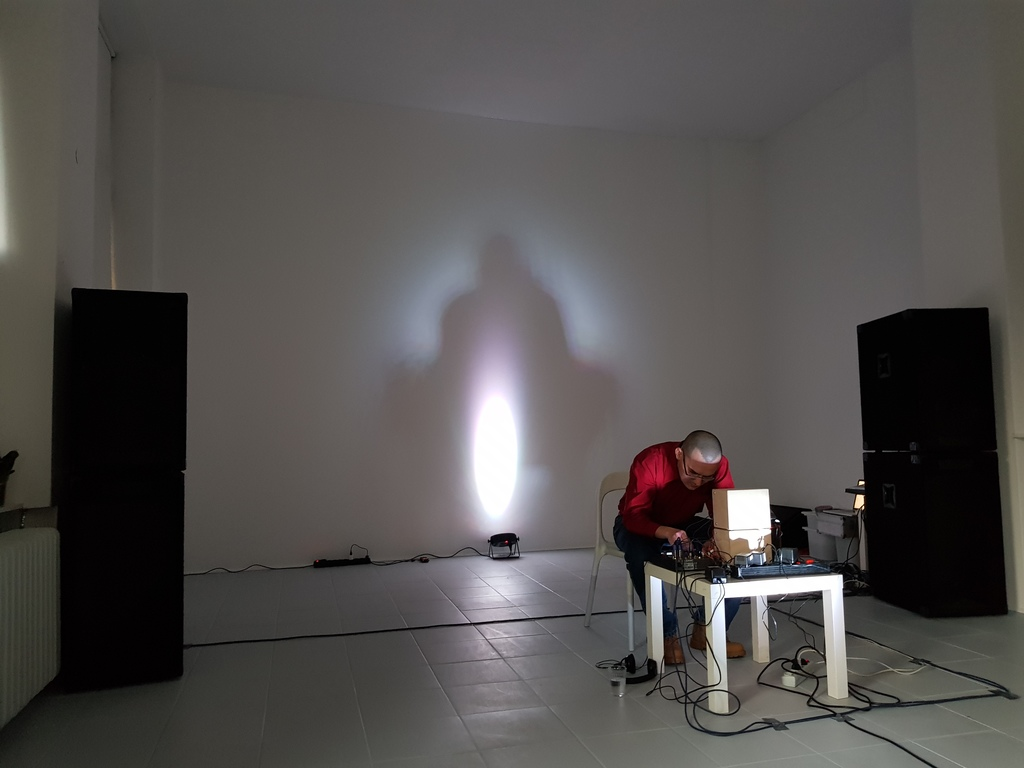
\includegraphics[width=0.99\textwidth]{calineczka-1maj.jpg}
  \caption*{RDS-2, 2017.05.01 -- photo by Jakub Klimek}
\end{wrapfigure}
\vspace{4mm}
\begin{wrapfigure}{l}{0.997\textwidth}
  \centering
  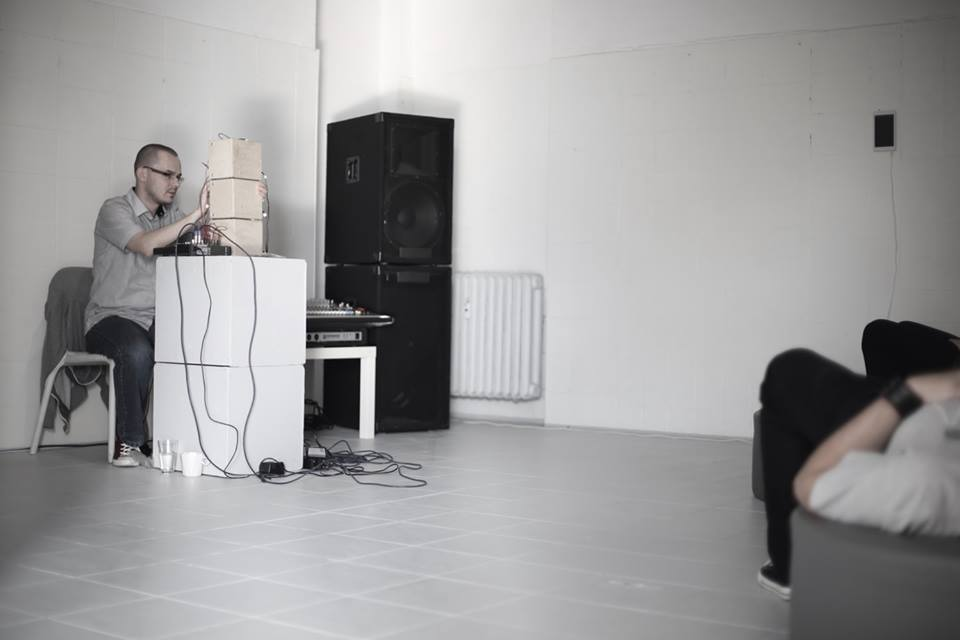
\includegraphics[width=0.99\textwidth]{calineczka-5h.jpg}
  \caption*{RDS-6, 2017.08.24 -- photo by Adam Mańkowski (\emph{Limited Liability Sounds})}
\end{wrapfigure}

%\newpage

\begin{wrapfigure}{l}{0.997\textwidth}
  \centering
  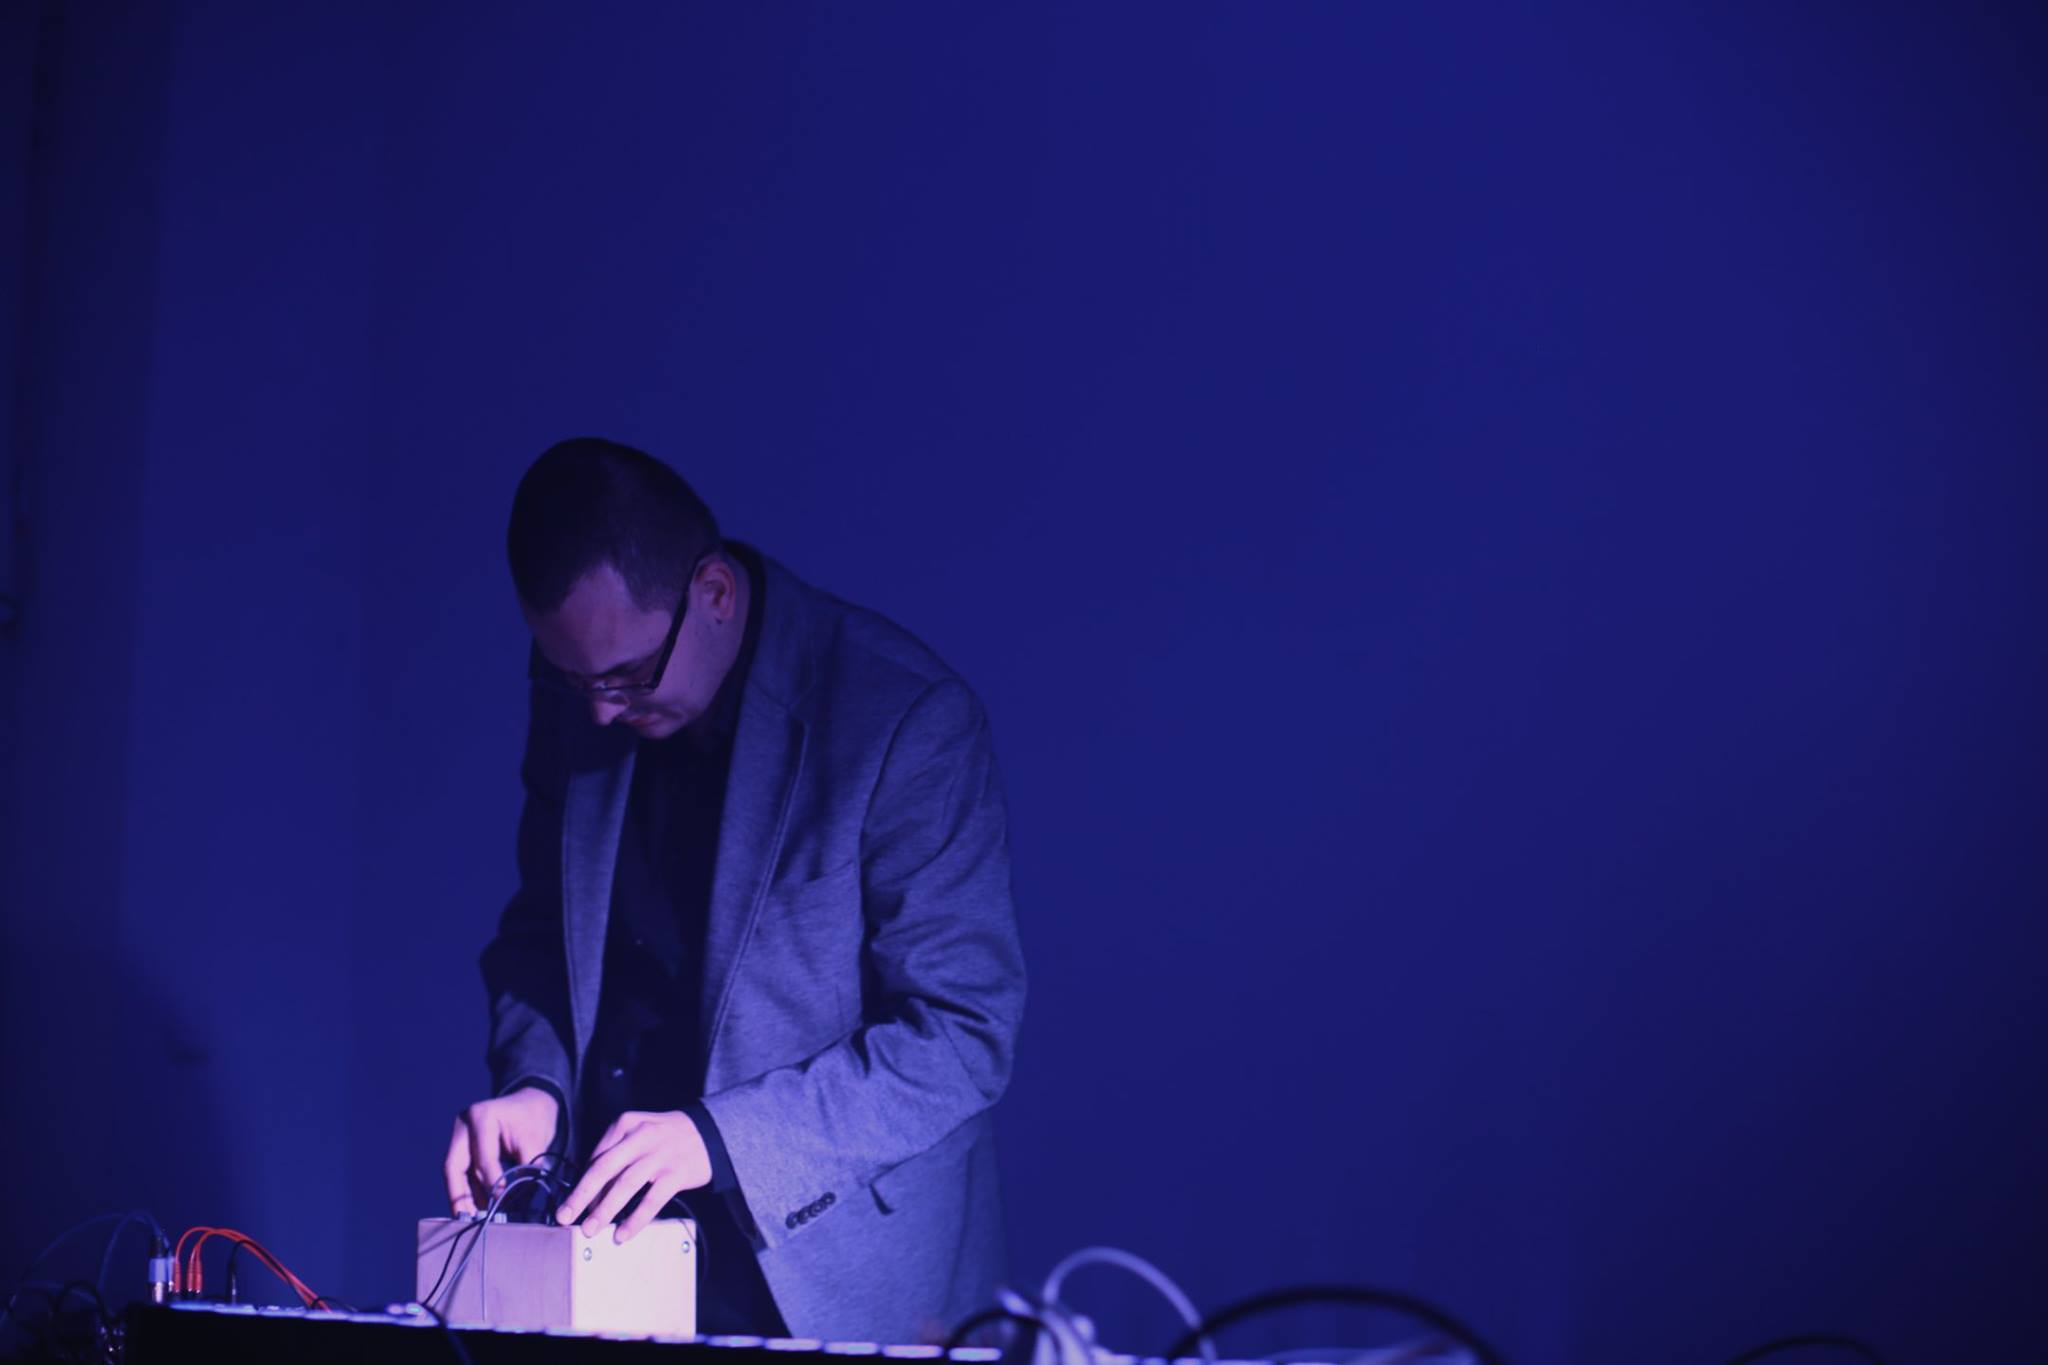
\includegraphics[width=0.99\textwidth]{calineczka-dnna.jpg}
  \caption*{RDS-9, 2019.01.26 -- photo by Sylwester Gałuszka (\emph{Kolonia Artystów})}
\end{wrapfigure}
\vspace{4mm}
\begin{wrapfigure}{l}{0.997\textwidth}
  \centering
  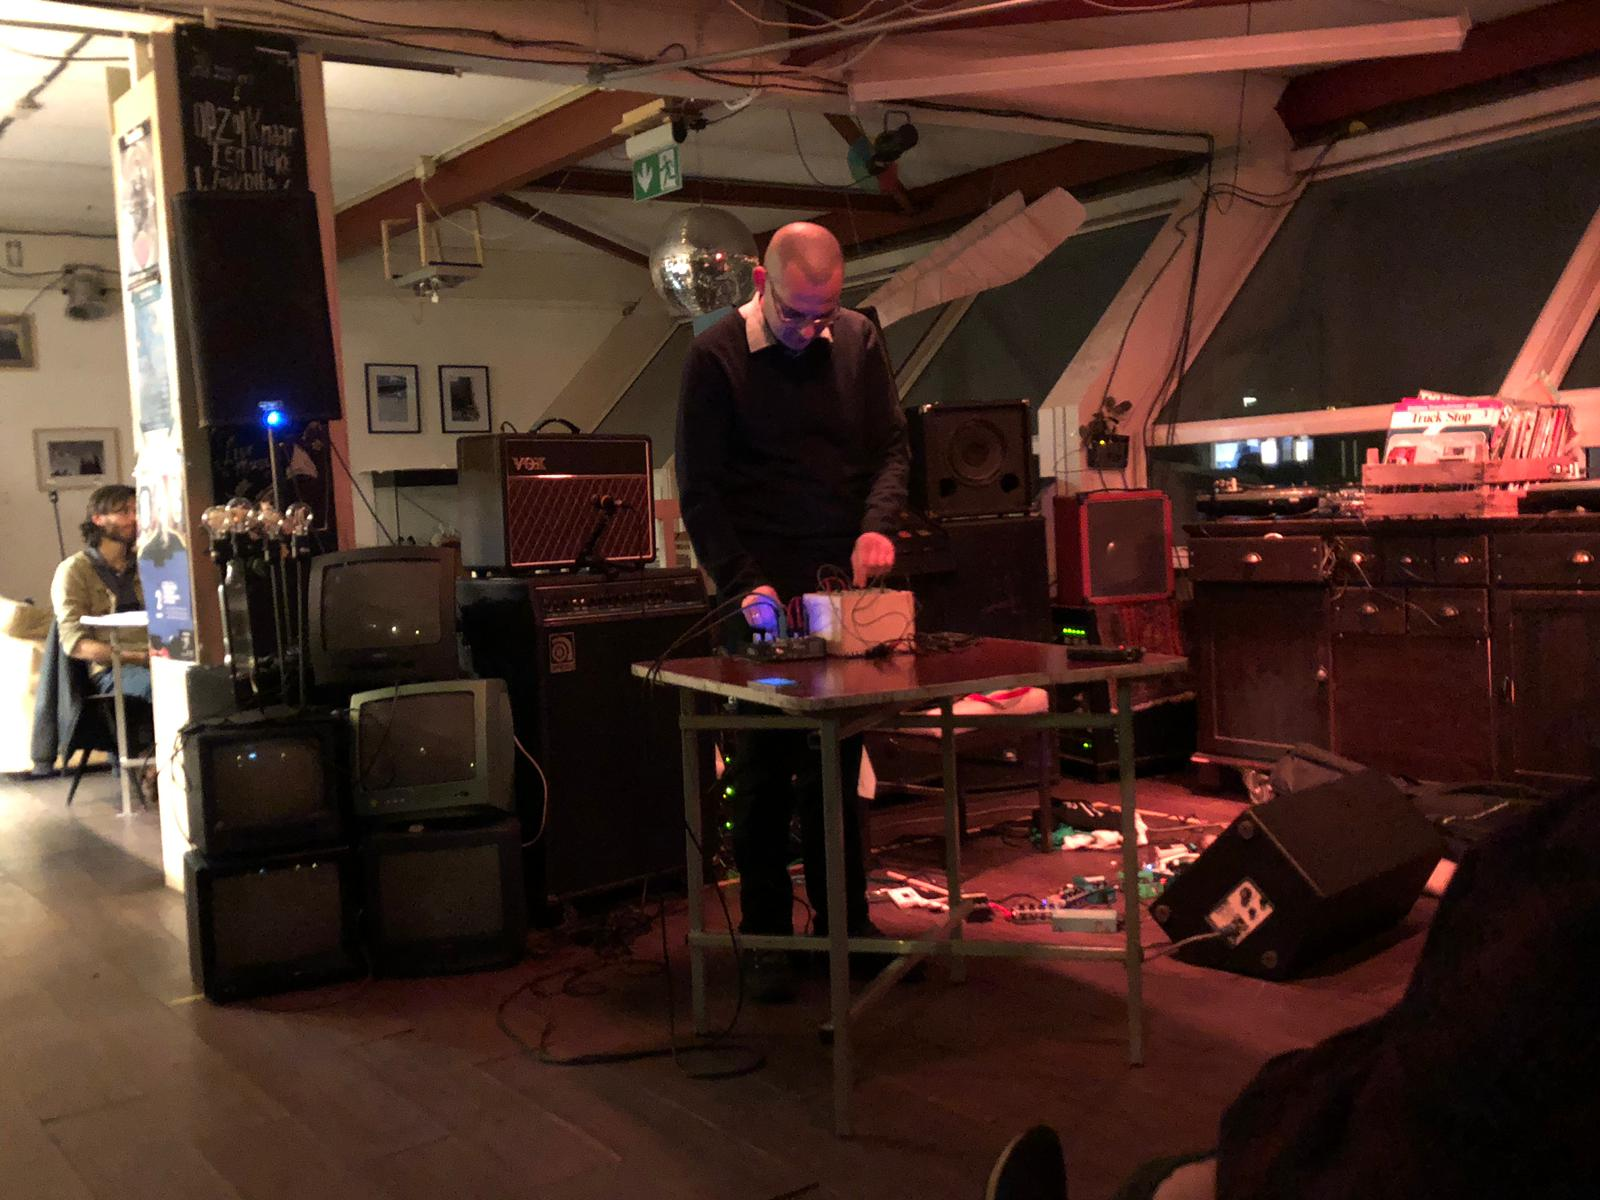
\includegraphics[width=0.99\textwidth]{calineczka-ams.jpg}
  \caption*{RDS-9, 2019.02.15 -- photo by Joey de Buck}
\end{wrapfigure}

%\newpage

\begin{wrapfigure}{l}{0.997\textwidth}
  \centering
  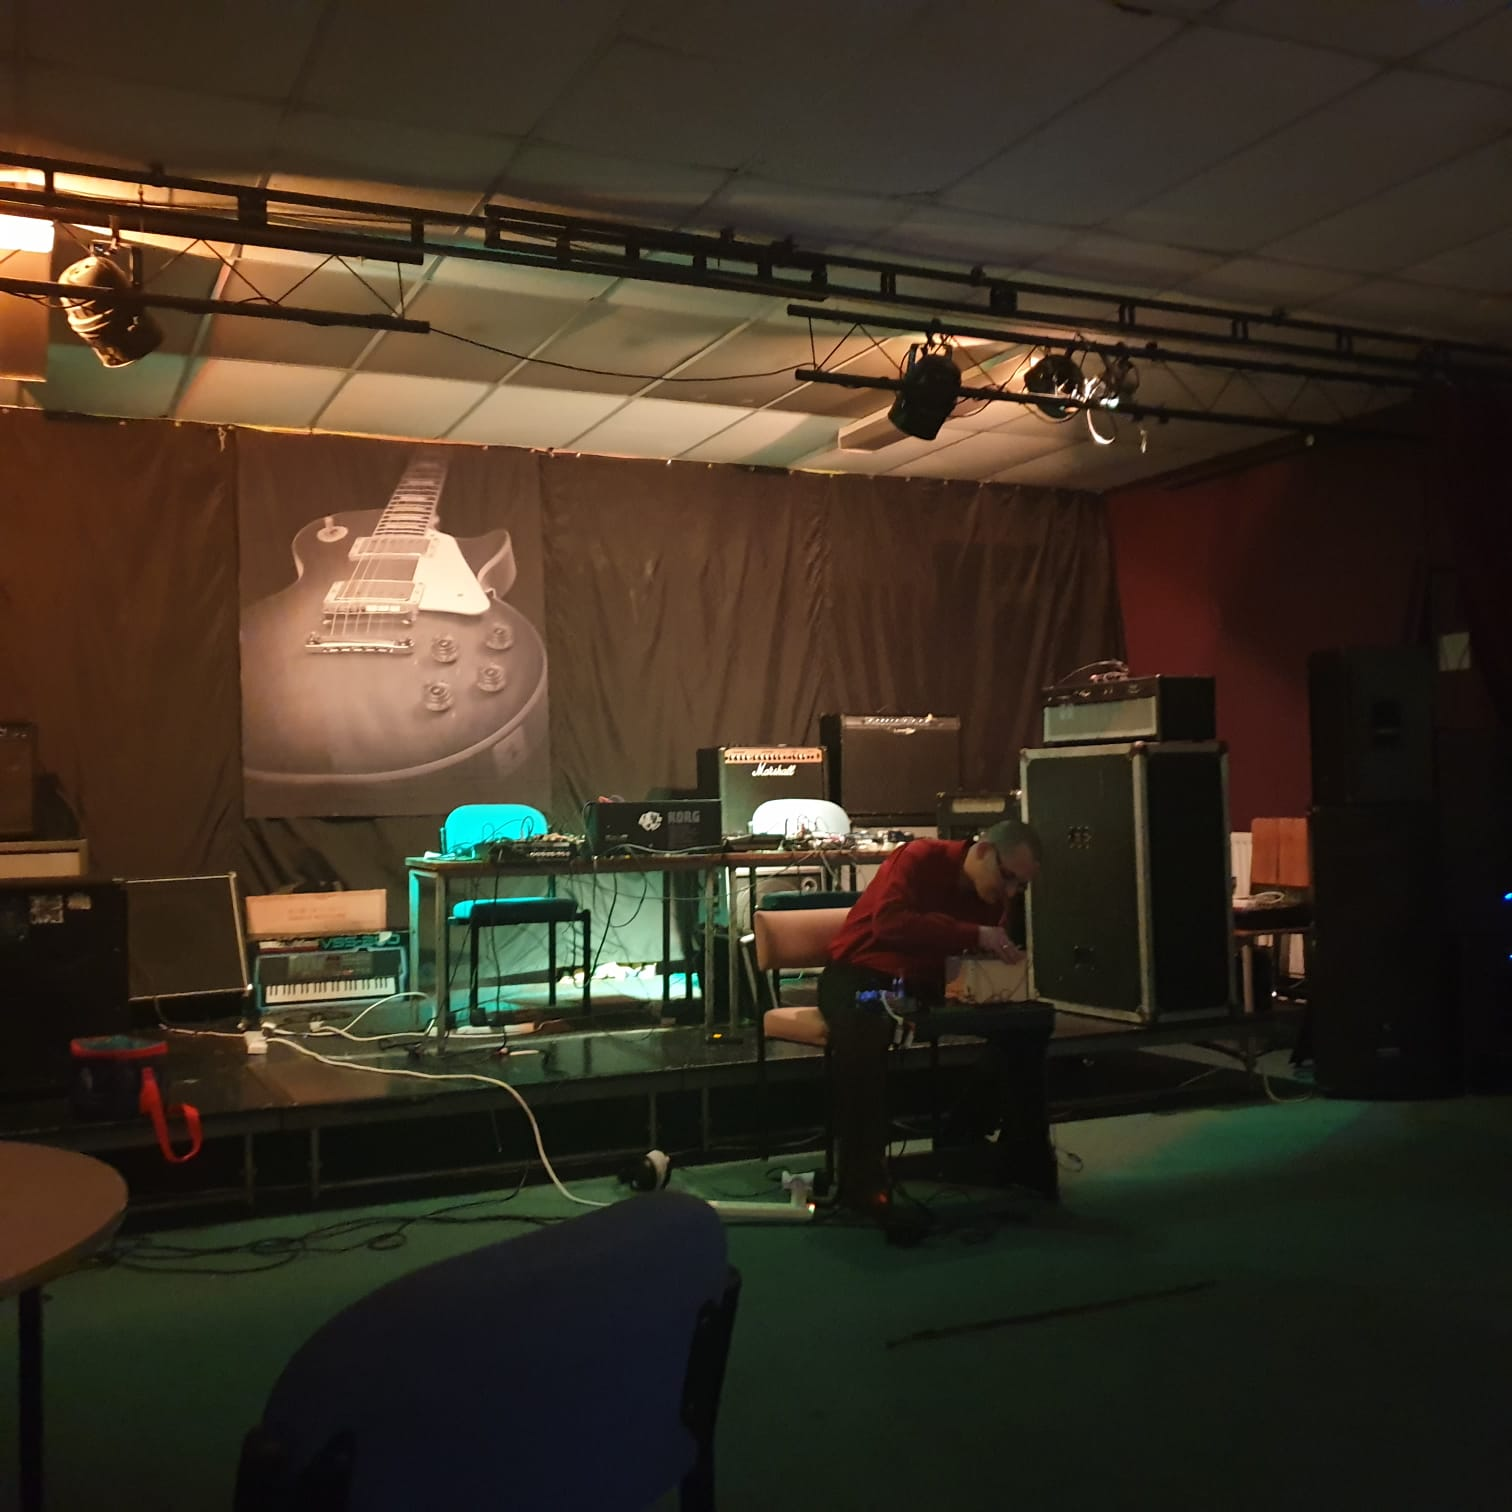
\includegraphics[width=0.99\textwidth]{calineczka-soundroom.jpg}
  \caption*{RDS-4, 2020.02.01 -- photo by Craig Stewart Johnson (\emph{Liminal Haze, Rovellasca})}
\end{wrapfigure}


\end{document}

